\section{\cphash{} Design}
\label{chap:mcstore}

As mentioned in Chapter \ref{chap:intro}, our goal is to create a scalable hash table 
that performs well on many core CPUs. To achieve such high scalability we use the idea of 
computation migration. Figure \ref{fig:mcstore} gives top level view of \cphash{} design. 
\cphash{} is split into multiple independent parts, which we call \textit{partitions}. We create a simple 
hash function to assign each possible key to a different partition. In \cphash{} all partitions are of equal size. Even though 
this might not always be the best idea, for simplicity we decided to keep it this way. 
If needed, partitions can be implemented to have a more flexible size by having more advanced 
memory management and data eviction algorithms (see Chapter \ref{chap:futurework} for discussion of such extensions).

Each partition has a designated server thread that is responsible for all operations 
on keys that belong to it. \cphash{} pin each server thread to its core.

\cphash{} is used in an application by having client threads that communicate with the server threads
and send queries using message passing (via shared memory). Server threads return query results
to the client threads also using message passing.  

\begin{figure}[!ht]
  \centering
  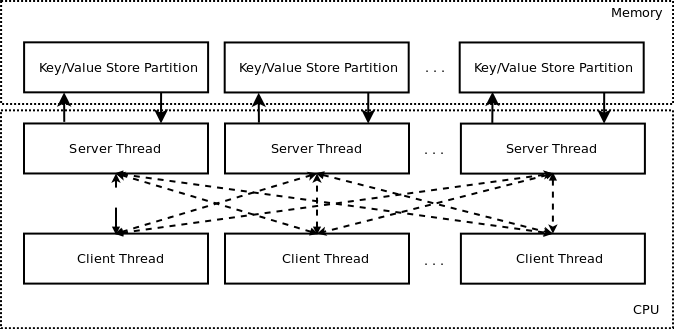
\includegraphics[width=0.8\linewidth]{figs/mcstore.png}
  \caption{\cphash{} Design}
  \label{fig:mcstore}
\end{figure}

  
Section \ref{sec:datastructure} below provides a more detailed description of the partition data structure. 
Sections \ref{sec:serverthreads} \ref{sec:clientthreads} describe the operation of the server and client threads in more detail. 
Section \ref{sec:msgpassing} describes our high performance message passing mechanism that uses buffering and batching. 
In Section \ref{sec:compmigration} we present benefits of computation migration. 

\subsection{Data Structure}
\label{sec:datastructure}

Every single partition in \cphash{} is a separate hash table. Figure \ref{fig:partition} shows the partition data structure.
Each partition contains a Bucket array. Each Bucket is a linked list. Keys are placed into different buckets based on a hash 
function that maps a key to a specific bucket. Each partition also has an LRU linked list that holds 
elements in the least recently used order. We use LRU list to determine which elements to evict from
a partition when there is not enough space left to insert new elements.

We pre-allocate the space that a partition can use to store data elements at initialization. 
Each element stored consists of a \texttt{key}, a \texttt{pointer} to a value, and a \texttt{size}. 
In \cphash{} the keys are limited to being 60-bit integer numbers; however, this can easily be 
extended to support any key size (see Section \ref{sec:anykey} for more details). 

\begin{figure}[!ht]
  \centering
  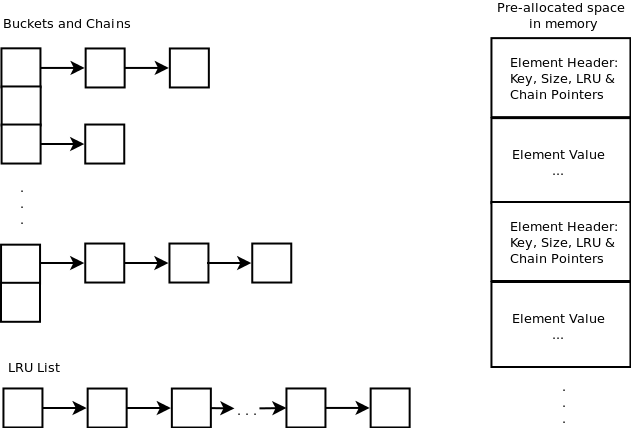
\includegraphics[width=0.8\linewidth]{figs/partition.png}
  \caption{Partition Data Structure}
  \label{fig:partition}
\end{figure}

\subsection{Server Threads}
\label{sec:serverthreads}

Each server thread is responsible for all the operations that are done on a single partition. 
The server thread continuously loops over the message queues of each client checking for new requests. When requests arrive, the 
server thread performs the requested operation and sends its result back to the client. 

\cphash{} supports two types of operations: \texttt{Lookup} and \texttt{Insert}. 
In the case of a \texttt{Lookup}, the message contains the requested \texttt{key}. If a key/value pair with the given 
\texttt{key} is found in the partition, then the server thread updates the head of the partition's LRU list and return the \texttt{pointer} to the 
value to the client thread; otherwise, the server returns a \texttt{NULL}.

Performing an \texttt{Insert} operation is slightly more complicated. \cphash{} is non-intrusive and 
supports arbitrary length values; thus, every time an insert operation occurs, space must be allocated 
in memory for the value to be copied over. In \cphash{}, the space for the value is allocated by the server 
thread but the data itself is copied by the client thread. Thus, to perform an \texttt{Insert} operation, the server needs 
to receive the \texttt{key} and the \texttt{size} of the data. The server thread allocates \texttt{size} amount of space and removes the existing 
key/value pair with the given \texttt{key} (if it exists) from the partition to avoid having duplicate keys for two different 
elements. The server returns a pointer to the allocated space to the client, which the client later fills in with the
actual data. Chapter 4 goes into more detail on how exactly the memory management works. 
  
\subsection{Client Threads}
\label{sec:clientthreads}

Applications have client threads that communicate with the server threads to get the queries done. 
Client threads do not necessarily have to be pinned to a specific core but, to achieve the highest performance 
in message passing, it is best to keep the client threads attached to a specific core. An example of a client 
thread in an application would be the client thread in \cpserver{} implementation. The client threads in \cpserver{} 
gather queries from the TCP connections, route them to the appropriate server threads, gather the results, and 
send them back to the correct TCP connections. Chapter \ref{chap:cpserver} describes the \cpserver{} implementation
in more detail.

\subsection{Buffering and Batching}
\label{sec:msgpassing}

\cphash{} implements message passing between the client and server threads using pre-allocated circular buffers in shared memory. 
For each server and client pair there are two buffers $-$ one for each direction of communication. Another possible way to 
implement message passing could have been to use single value communication. Figure \ref{fig:mpdesign} gives graphical representation for both designs.

In the single value communication pattern, space is allocated for each client/server pair and when a client wants to make 
a request to a server, it modifies this location with its query and waits for the server to respond. When the server is done processing the query it 
updates the shared location with the result. 

The implementation of a single one-way circular buffer consists of the following: a data buffer array, a read index, 
a write index, and a temporary write index. The buffer uses a single producer $-$ single consumer pattern. When the producer wants to add 
data to the buffer, it first makes sure that the read index is large enough compared to the temporary write index so that no 
unread data will be overwritten. Then it writes data to buffer and updates temporary write index. When the temporary write 
index is sufficiently larger than the write index, producer flushes the buffer by changing the write index to the temporary write index. 
To read data, the consumer waits until the read index is less than the write index, then it proceeds to read data and update the read 
index. The Read Index, Write Index and Temporary Write Index are carefully aligned in memory to avoid any false sharing. 
To decrease the number of cache misses when reading or writing buffers, the client threads flush the buffer when the whole cache line is 
full and the server threads update the read index after they are done reading all the queries in a cache line.

\begin{figure}[!ht]
  \centering
  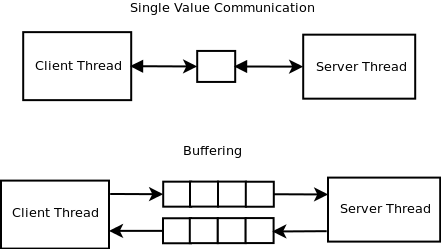
\includegraphics[width=0.8\linewidth]{figs/mpdesign.png}
  \caption{Message Passing Designs}
  \label{fig:mpdesign}
\end{figure}

There are two major benefits to using buffers instead of single value communication. The first advantage is improved parallelism. 
With buffers, the client can just queue the requests to the servers; thus, even if the server is busy, the client can continue working 
and schedule queries for other servers. This way all the servers can stay busy 100\% of the time, thus increasing the overall 
performance. The second reason is the decreased message passing overhead.  With single value communication, for every query 
received, the server would experience a cache miss; however, since the size of the cache line consists of multiple longs (in our test 
machines it is 64 bytes), with buffering the server can receive multiple requests using only a singe cache miss. Figure \ref{fig:mpdesign} 
shows the graphical representation of both designs.

With benefits there are some downsides to using buffers instead of the single value communication pattern. The circular buffer 
implementation requires having extra indices to enable the server and the client to know how much data has been written 
and how much has been read. Maintaining these indices introduces extra performance overhead that single value communication 
does not have. Thus, if the client sends requests to the server at a slow rate, single value communication would 
outperform the buffering implementation. However, if the client has a batch of requests that it needs to complete, buffering will be 
an advantage. Since we are improving the hash table data structure to target applications that are bottlenecked by 
the performance of the hash table, there should be no shortage of requests; therefore, buffering is a better design choice for 
message passing.

\subsection{Advantages of Computation Migration}
\label{sec:compmigration}

There are several advantages to using computation migration. The first advantage is having a better cache performance 
due to the fact that each partition is only modified and accessed by a single server thread, i.e. a single core. 
Since there is only one core accessing and modifying the data, there are no invalidations for data that 
is written. Furthermore, all frequently accessed structures, such as, the LRU list, buckets array, free list, etc can stay in 
the cache and can be read and modified fast. This provides a significant overall performance increase. 
Chapter \ref{chap:eval} reports on measurements that quantify the performance increase.

The second advantage is being able to get rid of synchronization mechanisms for shared data access and modification. 
Since each partition is modified by only a single core, there is no need for any synchronization mechanisms 
to protect the data from races. In addition to performance benefits, this approach also provides the benefit of ease of 
implementation. With computation migration the actual data structure operations are single threaded and, thus, no 
changes are necessary from the single threaded implementation. 

The more difficult part of the computation migration implementation lies with message passing; however, the message passing design 
and implementation can be standardized and the message passing design and implementation can stay exactly the same for many other data structures. 
Otherwise, to gain good scalability and performance for each specific data structure, different designs for synchronization would be 
necessary. For more complicated data structures the synchronization design can get very complicated with all 
possible cases of race conditions and data paths, thus leading to more potential implementation bugs. 
Computation migration provides an easier way to adopt a previous implementation of a single-threaded data structure 
into a more scalable one.

